\renewcommand{\one}{real_plastic-red-carton}
\renewcommand{\two}{real_cards-red}

\setlength{\raiseLen}{0.23in}
\setlength{\resLen}{0.52in}
\begin{figure*}[t]
	\addtolength{\tabcolsep}{-4pt}
	\begin{tabular}{cccc@{\hspace{4\tabcolsep}}ccc}
		& \textbf{\small SVBRDF maps} &
		\multicolumn{2}{c}{\textbf{\small Novel views}} &
		\textbf{\small SVBRDF maps} &
		\multicolumn{2}{c}{\textbf{\small Novel views}}
		\\
		\raisebox{\raiseLen}{\rotatebox[origin=c]{90}{\footnotesize{Ours (1)}}} &
		\includegraphics[height=\resLen]{results/multi_real/\one/ours+_1/tex.jpg} &
		\includegraphics[height=\resLen]{results/multi_real/\one/ours+_1/07.jpg} &
		\includegraphics[height=\resLen]{results/multi_real/\one/ours+_1/08.jpg} &
		\includegraphics[height=\resLen]{results/multi_real/\two/ours+_1/tex.jpg} &
		\includegraphics[height=\resLen]{results/multi_real/\two/ours+_1/07.jpg} &
		\includegraphics[height=\resLen]{results/multi_real/\two/ours+_1/08.jpg}
		\\
		\raisebox{\raiseLen}{\rotatebox[origin=c]{90}{\footnotesize{Ours (3)}}} &
		\includegraphics[height=\resLen]{results/multi_real/\one/ours+_3/tex.jpg} &
		\includegraphics[height=\resLen]{results/multi_real/\one/ours+_3/07.jpg} &
		\includegraphics[height=\resLen]{results/multi_real/\one/ours+_3/08.jpg} &
		\includegraphics[height=\resLen]{results/multi_real/\two/ours+_3/tex.jpg} &
		\includegraphics[height=\resLen]{results/multi_real/\two/ours+_3/07.jpg} &
		\includegraphics[height=\resLen]{results/multi_real/\two/ours+_3/08.jpg}
		\\
		\raisebox{\raiseLen}{\rotatebox[origin=c]{90}{\footnotesize{Ours (7)}}} &
		\includegraphics[height=\resLen]{results/multi_real/\one/ours+_7/tex.jpg} &
		\includegraphics[height=\resLen]{results/multi_real/\one/ours+_7/07.jpg} &
		\includegraphics[height=\resLen]{results/multi_real/\one/ours+_7/08.jpg} &
		\includegraphics[height=\resLen]{results/multi_real/\two/ours+_7/tex.jpg} &
		\includegraphics[height=\resLen]{results/multi_real/\two/ours+_7/07.jpg} &
		\includegraphics[height=\resLen]{results/multi_real/\two/ours+_7/08.jpg}
		\\
		\hline\\[-8pt]
		\raisebox{\raiseLen}{\rotatebox[origin=c]{90}{\footnotesize{Ours+ (1)}}} &
		\includegraphics[height=\resLen]{results/multi_real/\one/ours+_egsr_1/tex.jpg} &
		\includegraphics[height=\resLen]{results/multi_real/\one/ours+_egsr_1/07.jpg} &
		\includegraphics[height=\resLen]{results/multi_real/\one/ours+_egsr_1/08.jpg} &
		\includegraphics[height=\resLen]{results/multi_real/\two/ours+_egsr_1/tex.jpg} &
		\includegraphics[height=\resLen]{results/multi_real/\two/ours+_egsr_1/07.jpg} &
		\includegraphics[height=\resLen]{results/multi_real/\two/ours+_egsr_1/08.jpg}
		\\
		\raisebox{\raiseLen}{\rotatebox[origin=c]{90}{\footnotesize{Ours+ (3)}}} &
		\includegraphics[height=\resLen]{results/multi_real/\one/ours+_egsr_3/tex.jpg} &
		\includegraphics[height=\resLen]{results/multi_real/\one/ours+_egsr_3/07.jpg} &
		\includegraphics[height=\resLen]{results/multi_real/\one/ours+_egsr_3/08.jpg} &
		\includegraphics[height=\resLen]{results/multi_real/\two/ours+_egsr_3/tex.jpg} &
		\includegraphics[height=\resLen]{results/multi_real/\two/ours+_egsr_3/07.jpg} &
		\includegraphics[height=\resLen]{results/multi_real/\two/ours+_egsr_3/08.jpg}
		\\
		\raisebox{\raiseLen}{\rotatebox[origin=c]{90}{\footnotesize{Ours+ (7)}}} &
		\includegraphics[height=\resLen]{results/multi_real/\one/ours+_egsr_7/tex.jpg} &
		\includegraphics[height=\resLen]{results/multi_real/\one/ours+_egsr_7/07.jpg} &
		\includegraphics[height=\resLen]{results/multi_real/\one/ours+_egsr_7/08.jpg} &
		\includegraphics[height=\resLen]{results/multi_real/\two/ours+_egsr_7/tex.jpg} &
		\includegraphics[height=\resLen]{results/multi_real/\two/ours+_egsr_7/07.jpg} &
		\includegraphics[height=\resLen]{results/multi_real/\two/ours+_egsr_7/08.jpg}
		\\
		\hline\\[-8pt]
		\raisebox{\raiseLen}{\rotatebox[origin=c]{90}{\footnotesize{[Gao19]+ (1)}}} &
		\includegraphics[height=\resLen]{results/multi_real/\one/msra+_egsr_1/tex.jpg} &
		\includegraphics[height=\resLen]{results/multi_real/\one/msra+_egsr_1/07.jpg} &
		\includegraphics[height=\resLen]{results/multi_real/\one/msra+_egsr_1/08.jpg} &
		\includegraphics[height=\resLen]{results/multi_real/\two/msra+_egsr_1/tex.jpg} &
		\includegraphics[height=\resLen]{results/multi_real/\two/msra+_egsr_1/07.jpg} &
		\includegraphics[height=\resLen]{results/multi_real/\two/msra+_egsr_1/08.jpg}
		\\
		\raisebox{\raiseLen}{\rotatebox[origin=c]{90}{\footnotesize{[Gao19]+ (3)}}} &
		\includegraphics[height=\resLen]{results/multi_real/\one/msra+_egsr_3/tex.jpg} &
		\includegraphics[height=\resLen]{results/multi_real/\one/msra+_egsr_3/07.jpg} &
		\includegraphics[height=\resLen]{results/multi_real/\one/msra+_egsr_3/08.jpg} &
		\includegraphics[height=\resLen]{results/multi_real/\two/msra+_egsr_3/tex.jpg} &
		\includegraphics[height=\resLen]{results/multi_real/\two/msra+_egsr_3/07.jpg} &
		\includegraphics[height=\resLen]{results/multi_real/\two/msra+_egsr_3/08.jpg}
		\\
		\raisebox{\raiseLen}{\rotatebox[origin=c]{90}{\footnotesize{[Gao19]+ (7)}}} &
		\includegraphics[height=\resLen]{results/multi_real/\one/msra+_egsr_7/tex.jpg} &
		\includegraphics[height=\resLen]{results/multi_real/\one/msra+_egsr_7/07.jpg} &
		\includegraphics[height=\resLen]{results/multi_real/\one/msra+_egsr_7/08.jpg} &
		\includegraphics[height=\resLen]{results/multi_real/\two/msra+_egsr_7/tex.jpg} &
		\includegraphics[height=\resLen]{results/multi_real/\two/msra+_egsr_7/07.jpg} &
		\includegraphics[height=\resLen]{results/multi_real/\two/msra+_egsr_7/08.jpg}
	\end{tabular}
	\caption{\label{fig:results_multi_inputs}
		\textbf{Performance using different numbers of input images (real data).}
		\revision{The quality of SVBRDF maps recovered by our method generally improves with more input images under both constant initialization (see ``Ours'') and Deschaintre~\shortcite{Deschaintre2019} initialization (see ``Ours+'').}
	}
\end{figure*}